\documentclass{beamer}
\setcounter{errorcontextlines}{100}
%\usepackage[T1]{fontenc}
%\usepackage{charter}
\usepackage{graphicx}
\usepackage{eulervm}
\usepackage{amssymb,amsmath,amscd}
%\usepackage{colortbl}
\usepackage{comment}
\usepackage{multicol}

\usepackage{tikz}
\usepackage{listings}

\usepackage{color}
\usepackage{stmaryrd,bbm,mathtools}

\usetheme{Boadilla}
\usecolortheme{crane}
\useoutertheme{split}
\setbeamercolor{alerted text}{fg=red!80!craneorange!80!fg}
\setbeamersize{text margin left=2mm,text margin right=2mm}
\setbeamertemplate{navigation symbols}{}
\setbeamertemplate{blocks}[rounded][shadow=false]

%%%%%%%%%%% Some useful definitions

\newcommand{\thy}[1]{\texttt{#1}}
\newcommand{\C}{\mathbbm{C}}
\newcommand{\B}{\mathbbm{B}}
\newcommand{\E}{\mathbbm{E}}
\newcommand{\V}{\mathbbm{V}}
\newcommand{\N}{\mathbbm{N}}
\newcommand{\EmpThy}{\left\langle\,\right\rangle}

\newcommand{\semantics}[2]{\ensuremath{\llbracket{#2}\rrbracket_{#1}}}
\newcommand{\semC}[1]{\semantics{\B}{#1}}
\newcommand{\semE}[1]{\semantics{\E}{#1}}
\newcommand{\semP}[1]{\semantics{\pi}{#1}}
\newcommand{\partialf}{\rightharpoonup}

\newcommand{\ctx}[4]{\ensuremath{\left\langle #1:#2 \right\rangle_{#3}^{#4}}}
\newcommand{\ren}[4]{\ensuremath{\left[ #1\mapsto #2 \right]_{#3}^{#4}}}
\newcommand{\ctxcat}{\fatsemi}

\newcommand{\tmop}[1]{\ensuremath{\operatorname{#1}}}
\newcommand{\tmtexttt}[1]{{\ttfamily{#1}}}
\newcommand{\assign}{:=}
\newcommand{\tmdfn}[1]{\textbf{#1}}

\def\sem#1{\llbracket #1 \rrbracket}

\newbox\gnBoxA
\newdimen\gnCornerHgt
\setbox\gnBoxA=\hbox{$\ulcorner$}
\global\gnCornerHgt=\ht\gnBoxA
\newdimen\gnArgHgt


\def\Syntax #1{%
  \setbox\gnBoxA=\hbox{$#1$}%
  \gnArgHgt=\ht\gnBoxA%
  \ifnum \gnArgHgt<\gnCornerHgt
    \gnArgHgt=0pt%
  \else
    \advance \gnArgHgt by -\gnCornerHgt%
  \fi
  \raise\gnArgHgt\hbox{$\ulcorner$} \box\gnBoxA %
    \raise\gnArgHgt\hbox{$\urcorner$}}

\definecolor{slidered}{rgb}{1,0,0}
\definecolor{slideblue}{rgb}{0,0,1}
\definecolor{slidepurple}{rgb}{0,1,1}
\definecolor{slidegray}{rgb}{0.5,0.5,0.5}
\newcommand{\highlight}[1]{\textcolor{slidered}{#1}}
\newcommand{\sred}[1]{\textcolor{slidered}{#1}}
\newcommand{\sblue}[1]{\textcolor{slideblue}{#1}}
\newcommand{\sgray}[1]{\textcolor{slidegray}{#1}}
\newcommand{\spurple}[1]{\textcolor{slidepurple}{#1}}

\lstdefinelanguage{metaocaml}
    {morekeywords={module,struct,sig,end,let,Some,None,code,ret,type,fun,
        val,float,list,match,with,when}}

\lstdefinelanguage{mathscheme}
    {morekeywords={Theory,combine,extended,by,type,over,axiom,leftDomain,
        implies,not,forall}}

\lstset{language=metaocaml,basicstyle=\small}

\usepackage{latex/agda}
\usepackage{catchfilebetweentags}

%% Unicode stuff
\DeclareUnicodeCharacter {10814}{\ensuremath{\fatsemi}}

\title[Metaprogramming Agda]{Metaprogramming Agda}
\author[Carette, Al-hassy, Sharoda, Kahl]
  {\Large Jacques Carette, Musa Al-hassy, Yasmine Sharoda, Wolfram Kahl}
\institute[McMaster]{McMaster University}

\begin{document}
\begin{frame}
\thispagestyle{empty}
\titlepage
\end{frame}

% Remember to put 'fragile' on slides that use certain features
%\begin{frame}[fragile]
%\end{frame}

\begin{frame}
\frametitle{The Problem}
\begin{columns}
  \hspace*{-2cm}
  \begin{column}{0.5\textwidth} 
    {\tiny \ExecuteMetaData[latex/AgdaMeta.tex]{theory} }
    {\tiny \ExecuteMetaData[latex/AgdaMeta.tex]{sig} }
  \end{column}
  \hspace*{-2cm}
  \begin{column}{0.5\textwidth}
    {\tiny \ExecuteMetaData[latex/AgdaMeta.tex]{hom}}
    {\vspace*{\fill}}
  \end{column}
\end{columns}


\end{frame}

\begin{frame}[t,fragile]
\frametitle{(Presentations of) Algebraic Theories}
\lstset{language=mathscheme,basicstyle=\small}
\begin{onlyenv}<1->
\begin{lstlisting}
Monoid := Theory { 
  U : type;
  * : (U, U) -> U;
  e : U;
  axiom rightIdentity_*_e : forall x:U. x*e = x;
  axiom leftIdentity_*_e : forall x:U. e*x = x;
  axiom associative_* : forall x,y,z:U. (x*y)*z=x*(y*z)}
\end{lstlisting}
\end{onlyenv}
\begin{onlyenv}<2>
\begin{lstlisting}
CommutativeMonoid := Theory { 
  U : type;
  * : (U, U) -> U;
  e : U;
  axiom rightIdentity_*_e : forall x:U. x*e = x;
  axiom leftIdentity_*_e : forall x:U. e*x = x;
  axiom associative_* : forall x,y,z:U. (x*y)*z=x*(y*z)
  axiom commutative_* : forall x,y,z:U. x*y=y*x}
\end{lstlisting}
\end{onlyenv}
\begin{onlyenv}<3>
\begin{lstlisting}
AdditiveMonoid := Theory { 
  U : type;
  + : (U, U) -> U;
  0 : U;
  axiom rightIdentity_+_0 : forall x:U. x+0 = x;
  axiom leftIdentity_+_0 : forall x:U. 0+x = x;
  axiom associative_+ : forall x,y,z:U. (x+y)+z=x+(y+z) }
\end{lstlisting}
\end{onlyenv}
\begin{onlyenv}<4>
\begin{lstlisting}
AdditiveCommutativeMonoid := Theory { 
  U : type;
  + : (U, U) -> U;
  0 : U;
  axiom rightIdentity_+_0 : forall x:U. x+0 = x;
  axiom leftIdentity_+_0 : forall x:U. 0+x = x;
  axiom associative_+ : forall x,y,z:U. (x+y)+z=x+(y+z)
  axiom commutative_+ : forall x,y,z:U. x+y=y+x}
\end{lstlisting}
\end{onlyenv}
\end{frame}

\begin{frame}[t,fragile]
\frametitle{Pseudo-Combinators for (presentations of) theories}
Following Burstall \& Goguen (OBJ); Kapur, Musser, Stepanov (Tecton)\\ \vspace*{5mm}
Extension:
\begin{lstlisting}
CommutativeMonoid := Monoid extended by {
  axiom commutative_* : forall x,y,z:U. x*y=y*x}
\end{lstlisting}
\pause
Renaming:
\begin{lstlisting}
AdditiveMonoid := Monoid[ * |-> +, e |-> 0 ]
\end{lstlisting}
\pause
Combination:
\begin{lstlisting}
AdditiveCommutativeMonoid := 
  combine AdditiveMonoid, CommutativeMonoid over Monoid
\end{lstlisting}
\end{frame}

\lstset{language=mathscheme,basicstyle=\scriptsize}
\begin{frame}[t,fragile]
\frametitle{Library fragment 1}
\begin{lstlisting}
MoufangLoop := combine Loop, MoufangIdentity over Magma
LeftShelfSig := Magma[ * |-> |> ]
LeftShelf := LeftDistributiveMagma [ * |-> |> ]
RightShelfSig := Magma[ * |-> <| ]
RightShelf := RightDistributiveMagma[ * |-> <| ]
RackSig := combine LeftShelfSig, RightShelfSig over Carrier
Shelf := combine LeftShelf, RightShelf over RackSig
LeftBinaryInverse := RackSig extended by {
    axiom leftInverse_|>_<| : forall x,y:U. (x |> y) <| x = y }
RightBinaryInverse := RackSig extended by {
    axiom rightInverse_|>_<| : forall x,y:U. x |> (y <| x) = y }
Rack := combine RightShelf, LeftShelf, LeftBinaryInverse, 
    RightBinaryInverse over RackSig
LeftIdempotence := IdempotentMagma[ * |-> |> ]
RightIdempotence := IdempotentMagma[ * |-> <| ]
LeftSpindle := combine LeftShelf, LeftIdempotence over LeftShelfSig
RightSpindle := combine RightShelf, RightIdempotence over RightShelfSig
Quandle := combine Rack, LeftSpindle, RightSpindle over Shelf
\end{lstlisting}
\end{frame}

\begin{frame}[t,fragile]
\frametitle{Library fragment 2}
\begin{lstlisting}
NearSemiring := combine AdditiveSemigroup, Semigroup, RightRingoid over RingoidSig
NearSemifield := combine NearSemiring, Group over Semigroup
Semifield := combine NearSemifield, LeftRingoid over RingoidSig
NearRing := combine AdditiveGroup, Semigroup, RightRingoid over RingoidSig
Rng := combine AbelianAdditiveGroup, Semigroup, Ringoid over RingoidSig
Semiring := combine AdditiveCommutativeMonoid, Monoid1, Ringoid, Left0 over Ringoid0Sig
SemiRng := combine AdditiveCommutativeMonoid, Semigroup, Ringoid over RingoidSig
Dioid := combine Semiring, IdempotentAdditiveMagma over AdditiveMagma
Ring := combine Rng, Semiring over SemiRng
CommutativeRing := combine Ring, CommutativeMagma over Magma
BooleanRing := combine CommutativeRing, IdempotentMagma over Magma
NoZeroDivisors := Ringoid0Sig extended by {
  axiom onlyZeroDivisor_*_0: forall x:U.
    ((exists b:U. x*b = 0) and (exists b:U. b*x = 0)) implies (x = 0) }
Domain := combine Ring, NoZeroDivisors over Ringoid0Sig
IntegralDomain := combine CommutativeRing, NoZeroDivisors over Ringoid0Sig
DivisionRing := Ring extended by {
  axiom divisible : forall x:U. not (x=0) implies 
    ((exists! y:U. y*x = 1) and (exists! y:U. x*y = 1)) }
Field := combine DivisionRing, IntegralDomain over Ring
\end{lstlisting}
\end{frame}

\begin{frame}[t]
\frametitle{A fraction of the Algebraic Zoo}
\vspace*{-0.8cm}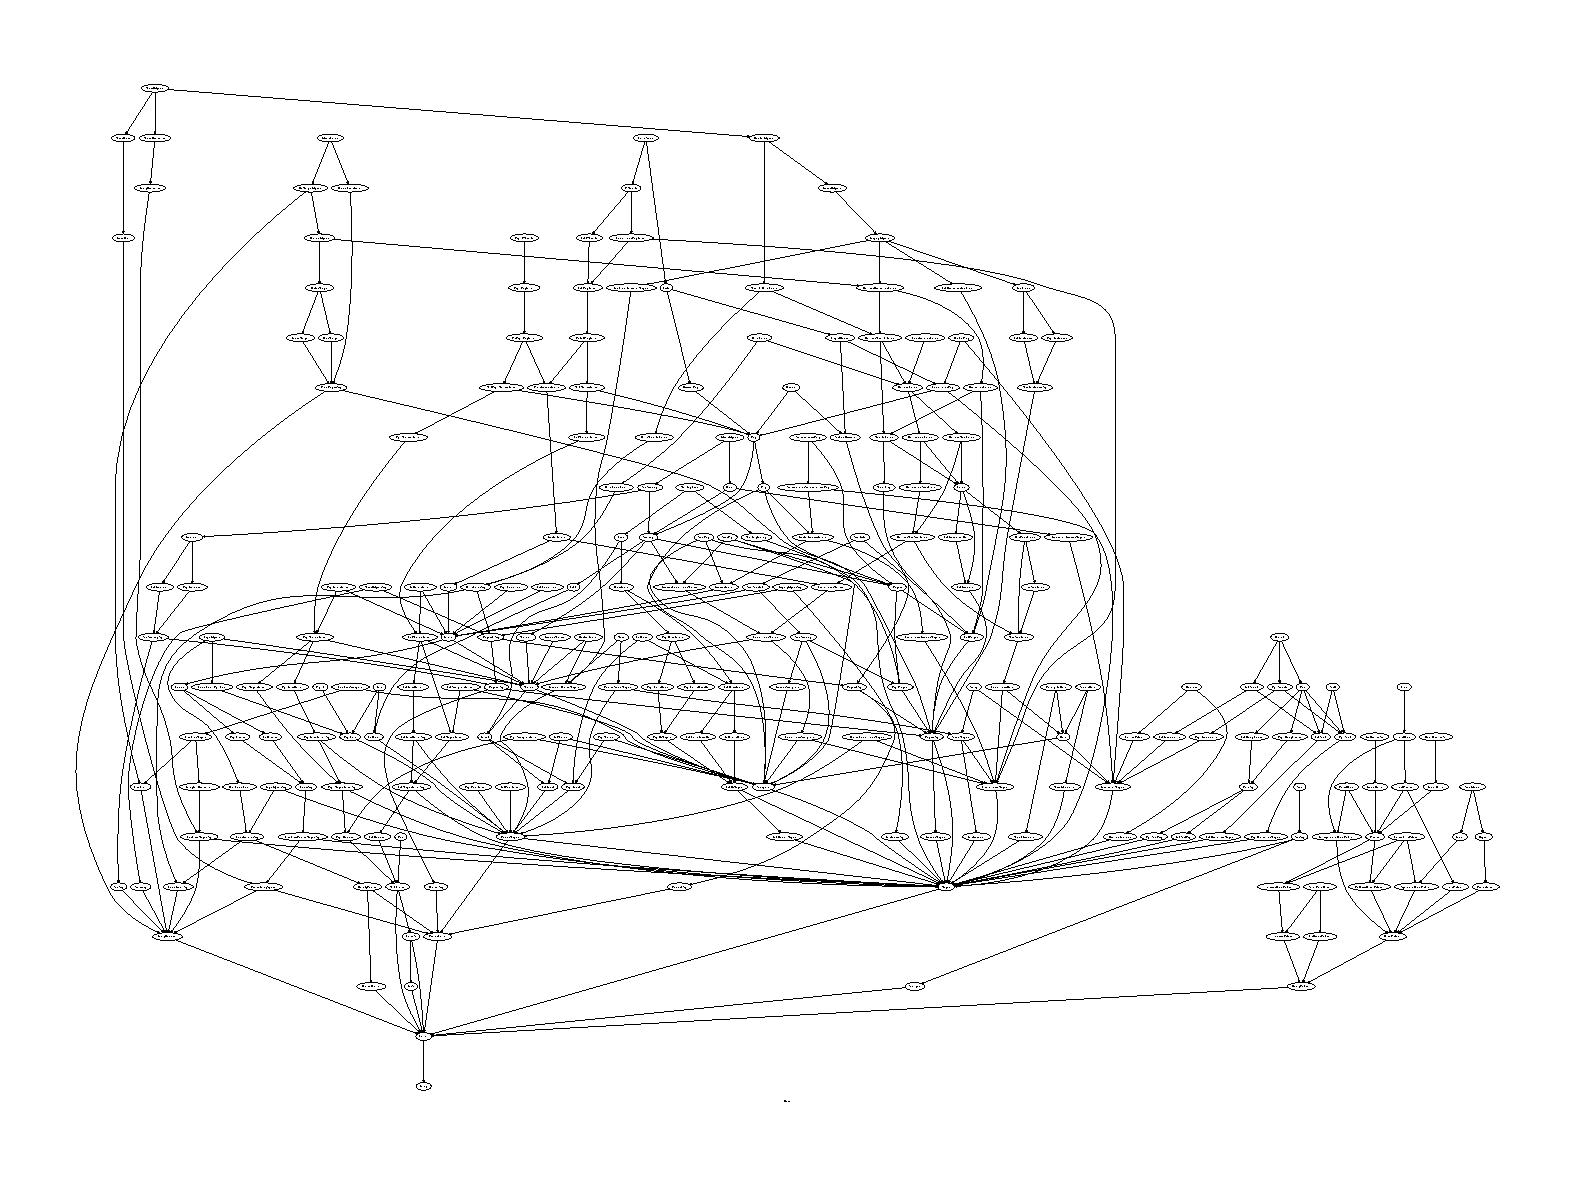
\includegraphics[height=9.5cm]{fragment.pdf}
\end{frame}

\lstset{language=mathscheme,basicstyle=\scriptsize}
\begin{frame}[t,fragile]
\frametitle{Biform monoids}
\begin{minipage}{6.6cm}
\begin{lstlisting}
Monoid := Theory { 
  U : type;
  e : U;
  * : (U, U) -> U;
  ax: forall x:U. e*x = x;
  ax: forall x:U. x*e = x;
  ax: forall x,y,z:U.(x*y)*z=x*(y*z)}
\end{lstlisting}
\end{minipage}
\begin{minipage}{5.3cm}
Syntax (term language)
\begin{lstlisting}[language=mathscheme,basicstyle=\ttfamily\scriptsize\color{red}]
MonoidTerm := Theory {
  type MTerm = (data X . 
    #e : X | 
    #* : (X, X) -> X)
}


\end{lstlisting}
\end{minipage}
\pause
Biform Theory: axiomatic + syntactic theory + transformers.\\
\hspace*{-1cm}
\begin{columns}[T]
\begin{column}{7.0cm}
\begin{visibleenv}<2->
\begin{lstlisting}
length :: MTerm -> Nat
length trm = gfold (+) 1 trm
\end{lstlisting}
\end{visibleenv}
\begin{onlyenv}<3>
\begin{lstlisting}
leftSimp  :: MTerm -> MTerm
leftSimp  = fun (#*(a,b)) when a = #e -> b
rightSimp :: MTerm -> MTerm
rightSimp = fun (#*(a,b)) when b = #e -> b
\end{lstlisting}
\end{onlyenv}
\begin{onlyenv}<4->
\begin{lstlisting}
simp :: MTerm -> MTerm
simp t = match t with
 | (#* (a,b)) when a = #e -> b
 | (#* (a,b)) when b = #e -> b
 | _                      -> t
\end{lstlisting}
\end{onlyenv}
\end{column}
\begin{column}{3.5cm}
\begin{visibleenv}<5->
\alert{Generic\\}
\vspace*{0.9cm}
\alert{Derived from length reducing axioms}
\end{visibleenv}
\end{column}
\end{columns}
%\begin{visibleenv}<6->
%``Homomorphism'' on theory presentations.  Modular?
%\end{visibleenv}
\end{frame}

\lstset{language=mathscheme,basicstyle=\scriptsize}
\begin{frame}[t,fragile]
\frametitle{Different interpretations of theories
\footnote{\scriptsize \textit{simplified MetaOCaml for clarity}}
}
\begin{minipage}{6.8cm}
\begin{lstlisting}
Monoid := Theory { 
  U : type;
  e : U;
  * : (U, U) -> U;
  ax: forall x:U. e*x = x;
  ax: forall x:U. x*e = x;
  ax: forall x,y,z:U.(x*y)*z=x*(y*z)}
\end{lstlisting}
\end{minipage}
\lstset{language=metaocaml,basicstyle=\scriptsize}
\begin{minipage}{5.4cm}
Monoid type, as values
\begin{lstlisting}
module type MONOID = sig
  type n
  val plus : n -> n -> n
  val zero : n
end

\end{lstlisting}
\end{minipage}
\vspace*{.3cm}\hspace*{-.3cm}
\begin{columns}[T]
\begin{column}{6.0cm}
\begin{onlyenv}<2-3>
Monoid type, as code
\begin{lstlisting}
module type MONOIDCODE = sig
  type n
  type nc = n code
  val plus : nc -> nc -> nc
  val zero : nc
end

\end{lstlisting}
\end{onlyenv}
\end{column}
\begin{column}{5.5cm}
\begin{onlyenv}<3-3>
Monoid type, staged
\begin{lstlisting}
type x staged = Now of x 
              | Later of x code
module type MONOIDSTAGED = sig
  type n
  type ns = n staged
  val plus : ns -> ns -> ns
  val zero : ns
end
\end{lstlisting}
\end{onlyenv}
\end{column}
\end{columns}
\end{frame}

\begin{frame}[t,fragile]
\frametitle{From syntax to code}
\begin{minipage}{5.4cm}
\lstset{language=mathscheme,basicstyle=\scriptsize}
\begin{lstlisting}
MonoidTerm := Theory {
  type MTerm = (data X . 
    #e : X | 
    #* : (X, X) -> X)
}


\end{lstlisting}
\end{minipage}
\lstset{language=metaocaml,basicstyle=\scriptsize}
\begin{minipage}{5.4cm}
\begin{lstlisting}
module type MONOIDSTAGED = sig
  type n
  type ns = n staged
  val zero : ns
  val plus : ns -> ns -> ns
end
\end{lstlisting}
\end{minipage}
\vspace*{.3cm}\hspace*{-.7cm}
\begin{columns}[T]
\begin{column}{5.5cm}
\begin{visibleenv}<2>
Equality is ``free''\\
\lstset{language=mathscheme,basicstyle=\scriptsize}
\begin{lstlisting}
simp :: MTerm -> MTerm
simp t = match t with
 | (#* (a,b)) when a = #e -> b
 | (#* (a,b)) when b = #e -> b
 | _                      -> t

\end{lstlisting}
\end{visibleenv}
\end{column}
\begin{column}{5.8cm}
\begin{visibleenv}<2>
Equality is ``now''\\
\lstset{language=metaocaml,basicstyle=\scriptsize}
\begin{lstlisting}
let monoid zero plusN plusL x y = 
  match x, y with
  | (Now a), b when a = zero -> b
  | a, (Now b) when b = one -> a
  | _  -> lift2 plusN plusL x y
\end{lstlisting}
\end{visibleenv}
\end{column}
\end{columns}
\end{frame}

\lstset{language=metaocaml,basicstyle=\scriptsize}
\begin{frame}[t,fragile]
\frametitle{Concrete Monoids}
\begin{minipage}{5.4cm}
\begin{lstlisting}
module IntM = struct
  type n = Int
  let plus = (+)
  let zero = 0
end
\end{lstlisting}
\end{minipage}
\begin{minipage}{5.4cm}
\begin{lstlisting}
module IntMC = struct
  type n = Int
  type 'a nc = ('a,n) code
  let plus = .<fun x y -> .~x + .~y>.
  let zero = .< 0 >.
end
\end{lstlisting}
\end{minipage}
\vspace*{.3cm}
\begin{lstlisting}
module IntMS = struct
  type n = Int
  type 'a ns = ('a,n) staged
  let plus = monoid IntM.zero IntM.plus IntMC.plus
  let zero = Now IntM.zero
end
\end{lstlisting}
\pause
\begin{block}{Machinery for free}
Given a structured graph of theories, one can get a (na\"{\i}ve)
optimizing compiler.
\end{block}
\end{frame}

\lstset{mathescape,basicstyle=\ttfamily\fontsize{2.5pt}{3pt}\selectfont}
\begin{frame}[fragile,t]
\begin{multicols}{3} 
     \begin{minipage}{2.3in}
\underline{MSL}
\begin{lstlisting}
Monoid := Theory {
 U : type; 
 * : (U,U) -> U; 
 e : U; 
 axiom right_identity_*_e : 
  forall x : U . (x * e) = x 
 axiom left_identity_*_e : 
  forall x : U . (e * x) = x;
 axiom associativity_* : 
  forall x,y,z : U . 
   ((x * y) * z) = (x * (y * z));
}
\end{lstlisting}
\underline{Coq}
\begin{lstlisting}
Class Monoid {A : type} 
 (dot : A -> A -> A)
 (one : A) : Prop := {
 dot_assoc : 
   forall x y z : A, 
     (dot x (dot y z)) 
     = dot (dot x y) z
 unit_left : 
  forall x, dot one x = x 
 unit_right : 
  forall x, dot x one = x 
}      
\end{lstlisting}
Alternative Definition: 
\begin{lstlisting}
Record monoid := { 
 dom : Type; 
 op : dom -> dom -> dom 
  where "x * y" := (op x y); 
 id : dom where "1" := id ;  
 assoc : forall x y z, x * (y * z) = (x * y) * z; 
 left_neutral : forall x, 1 * x = x; 
 right_neutral : forall x, x * 1 = x
}.
\end{lstlisting}
 \end{minipage}
  
\begin{minipage}{2.9in}
\underline{Haskell}
\begin{lstlisting}
class Semigroup a => Monoid a where 
 mempty :: a 
 mappend :: a -> a -> a 
 mappend = (<>) 
 mconcat :: [a] -> a 
 mconcat = foldr mappend mempty
\end{lstlisting}
\underline{Isabelle}
\begin{lstlisting}
class semigroup = 
 fixes mult :: $\alpha$ => $\alpha$ => $\alpha$
      (infixl $\otimes$ 70) 
 assumes assoc :: (x $\otimes$ y) $\otimes$ z
         = x $\otimes$ (y $\otimes$ z)
class monoidl = semigroup + 
 fixes neutral :: $\alpha$ ($\textbf{1}$)
 assumes neutl : $\textbf{1}$ $\otimes$ x = x 
class monoid = monoidl + 
 assumes x $\otimes$ $\textbf{1}$ = x
\end{lstlisting}
\underline{Lean}
\begin{lstlisting}
universe u 
variables{ $\alpha$ : Type u }
class monoid ($\alpha$ : Type u) extends
  semigroup $\alpha$, has_one $\alpha$ := 
  (one_mul : $\forall$ a : $\alpha$, 1 * a = a)
  (mul_one : $\forall$ a : $\alpha$, a * 1 = a)
\end{lstlisting}
        \end{minipage} 
        \begin{minipage}{3in}
\underline{Agda}
\begin{lstlisting}
data Monoid (A : Set) 
  (Eq : Equivalence A) : Set 
where 
 monoid : 
  (z : A)
  (_+_ : A -> A -> A)
  (left_Id : LeftIdentity Eq z _+_)
  (right_Id : RightIdentity Eq z _+_)  
  (assoc : Associative Eq _+_) -> 
  Monoid A Eq 
\end{lstlisting}
Alternative Definition: 
\begin{lstlisting}
record Monoid c $\ell$ : 
 Set (suc (c $\sqcup$ $\ell$)) where 
 infixl 7 _$\bullet$_ 
 infix 4 _$\approx$_ 
 field 
  Carrier : Set c 
  _$\approx$_ : Rel Carrier $\ell$ 
  _$\bullet$_ : Op$_2$ Carrier 
  isMonoid : 
  IsMonoid _$\approx$_ _$\bullet$_ $\epsilon$ 
\end{lstlisting}
where
\begin{lstlisting}
record IsMonoid ($\bullet$ : Op$_2$) ($\varepsilon$ : A) 
   : Set (a $\sqcup$ $\ell$) where 
 field 
  isSemigroup : IsSemigroup $\bullet$ 
  identity : Identity $\varepsilon$ $\bullet$ 
       
  identity$^l$ : LeftIdentity $\varepsilon$ $\bullet$ 
  identity$^l$ = proj$_1$ identity 
        
  identity$^r$ : RightIdentity $\varepsilon$ $\bullet$ 
  identity$^r$ = proj$_2$ identity 
\end{lstlisting}
       \end{minipage}
  \end{multicols} 
\end{frame}

\begin{frame}
\frametitle{Universal Algebra...}
Most of these work for Generalized Algebraic Theories (\`{a} la Cartmell):
\begin{itemize}
\item Signature
\item Term Algebra
\begin{itemize}
\item ``generic functions'' (\`{a} la \textit{Scrap your Boilerplate})
\item Structural induction
\end{itemize}
\item Term Algebra parametrized by a ``theory'' of variables
\begin{itemize}
\item predicate for ground terms
\item ``simplifier'' for open terms (correct but usually incomplete)
\end{itemize}
\item \sred{Homomorphism}; homomorphism composition; isomorphism
\item kernel of homomorphism
\item Theory of congruence relations over a theory
\item Induced congruence of a homomorphism 
\item Interpreter from Term Algebra to any instance of a theory
\item Partial evaluator
\item Sub-theory, Product Theory, Co-product Theory
\item Internalization (making a record that represents a theory)
\end{itemize}
\end{frame}

\end{document}

%%%%%%%%%%%%%%%%%%%%%%%%%%%%%%%%%%%%%%%%%%%%%%%%%%%%%%%%%%%%%%%%%%%%%%%%%
